\chapter{Геометрические вероятности}

\section*{Введение}

Геометрическое определение вероятности является обощение классического определения на случай несчетных множеств элементарных исходов $\Omega$. Предполагается наличие некоторой
"геометрической"{} меры $\mu$, определенной для всех событий $A \in S$ алгебры событий $S$ (в том числе и для $\Omega \in S$). С помощью меры $\mu$ вводится вероятностная мера
$P$:
\begin{equation}
    P \left ( A \right ) = \frac{\mu \left ( A \right )}{\mu \left ( \Omega \right )}.
\end{equation}

Как правило, в качестве меры $\mu$ на практике выступает понятия длины, площади, объёма.

\section*{Задача 18.140}

Внутри квадрата с вершинами (0, 0), (1, 0), (1, 1) и (0, 1) наудачу выбирается точка $M(x,y)$. Найти вероятность события $B = \event{(x, y) | xy < a, a > 0}$.

\subsection*{Решение:}

В данном случае множество всех элементарных исходов представляет собой точки квадрата:
\begin{equation}
    \Omega = \left \{ (x, y) : 0 \le x, y \le 1 \right \}.
\end{equation}

В качестве "геометрической"{} меры $\mu$ используется площадь, поэтому
\begin{equation}
    \mu \left ( \Omega \right ) = 1.
\end{equation}

Форма события $B$ зависит от значения параметра $a$.
\begin{enumerate}
    \item
    Если $a > 1$, то все точки $(x,y)$ квадрата $\Omega$ удовлетворяют условию $x y < a$, поэтому
    \begin{equation}
        B = \Omega,
    \end{equation}
    и вероятность события $B$:
    \begin{equation}
        \probability{B}
        = \frac{\mu \left ( B \right )}{\mu \left ( \Omega \right )}
        = \frac{\mu \left ( \Omega \right )}{\mu \left ( \Omega \right )}
        = 1 .
    \end{equation}

    \item
    Если $0 < a \le 1$, тогда множество точек $B$ можно представить в виде объединения двух непересекающихся множеств (рисунок \ref{figure:lesson_3:40:B}):
    \begin{equation}
        B = B_1 + B_2 ,
    \end{equation}
    где $B_1$ --- прямоугольное множество и $B_2$ --- множество точек под гиперболой.

    \begin{figure}[h]
        \centering
        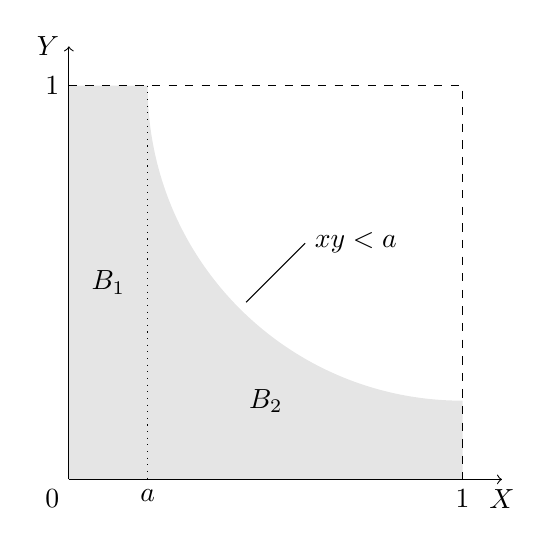
\begin{tikzpicture}[scale=5]
            \def \a {0.2};
            % фигура события
            \path [fill=gray!20] ( 0, 0 ) -- ( 0, 1 ) -- ( \a, 1 ) to [out=-90,in=180] ( 1, \a ) -- ( 1, 0 ) -- ( 0, 0 );
            \draw ( 0.45, 0.45 ) -- ( 0.6, 0.6 ) node [right] ( 0.6, 0.6 ) {$xy < a$};

            % оси
            \draw [->] ( 0, 0 ) -- ( 1.1, 0 ) node [below] at ( 1.1, 0 ) {$X$};
            \draw [->] ( 0, 0 ) -- ( 0, 1.1 ) node [left] at ( 0, 1.1 ) {$Y$};
            \node [below left] at ( 0, 0 ) {$0$};
            \node [below] at ( 1, 0 ) {$1$};
            \node [left] at ( 0, 1 ) {$1$};

            % границы квадрата
            \draw [dashed] ( 0, 1 ) -- ( 1, 1 ) -- ( 1, 0 );
            \draw [dotted] ( \a, 1 ) -- ( \a, 0 ) node [below] at ( \a, 0 ) {$a$};
            \node at ( 0.1, 0.5) {$B_1$};
            \node at ( 0.5, 0.2) {$B_2$};
        \end{tikzpicture}
        \caption{Событие $B = B_1 + B_2$.}
        \label{figure:lesson_3:40:B}
    \end{figure}

    Мера множества $B_1$ легко вычисляется --- это площадь прямоугольника:
    \begin{equation}
        \mu \left ( B_1 \right )
        = 1 \cdot a
        = a .
    \end{equation}

    Мера множества $B_2$ --- площадь под гиперболой $y = \frac{a}{x}$:
    \begin{equation}
        \mu \left ( B_2 \right )
        = \int \limits_{a}^1 \frac{a}{x} dx
        = \left . a \ln x \right |_a^1
        = a \left ( \ln 1 - \ln a \right )
        = - a \ln a .
    \end{equation}

    Вероятность события $B$:
    \begin{equation}
        \probability{B}
        = \frac{\mu \left ( B \right )}{\mu \left ( \Omega \right )}
        = \frac{\mu \left ( B_1 + B_2 \right )}{\mu \left ( \Omega \right )}
        = \frac{\mu \left ( B_1 \right ) + \mu \left ( B_2 \right )}{\mu \left ( \Omega \right )}
        = \frac{a - a \ln a}{1}
        = a \left ( 1 - \ln a \right ).
    \end{equation}
\end{enumerate}

\subsection*{Ответ:}
$
\probability{B} =
\left \{
\begin{array}{ll}
    a \left ( 1 - \ln a \right ), & 0 < a \le 1 \\
    1,                            & 1 < a
\end{array}
\right .
.
$

\section*{Задача 18.143}

Какова вероятность того, что сумма трех наудачу взятых отрезков, длина каждого из которых не превосходит $l$, будет больше $l$.

\subsection*{Решение:}

Пусть $x$, $y$, $z$ обозначают длины отрезков. Множество всех элементарных исходов:
\begin{equation}
    \Omega = \set{(x, y, z) : 0 \le x, y, z \le l}
\end{equation}
представляет собой куб с длиной ребра равной $l$.

В качестве геометрической меры $\mu$ возьмем объём. При таком определении геометрическая мера $\Omega$:
\begin{equation}
    \mu \left ( \Omega \right ) = l^3.
\end{equation}

Пусть $A$ обозначает событие, при котором сумма длин отрезков больше $l$. В терминах принятых элементарных исходов:
\begin{equation}
    A = \set{(x,y,z) : x + y + z > l, 0 \le x, y, z \le l}.
\end{equation}

Для вычисления геометрической меры $A$ удобно использовать дополнительное событие --- $\overline{A}$:
\begin{gather}
    A + \overline{A} = \Omega , \\
    \mu \left ( A + \overline{A} \right ) = \mu \left ( \Omega \right ), \\
    \mu \left ( A \right ) + \mu \left ( \overline{A} \right ) = \mu \left ( \Omega \right ), \\
    \mu \left ( A \right ) = \mu \left ( \Omega \right ) - \mu \left ( \overline{A} \right ) .
\end{gather}

Событие $\overline{A}$:
\begin{equation}
    \overline{A} = \set{(x,y,z): x + y + z \le l, 0 \le x, y, z \le l} .
\end{equation}
представляет собой треугольную пирамиду, образованную плоскостями (рисунок \ref{figure:lesson_3:143:cube}):
\begin{gather}
    x + y + z = l, \\
    x = 0, \\
    y = 0, \\
    z = 0 .
\end{gather}

\begin{figure}[h]
    \centering
    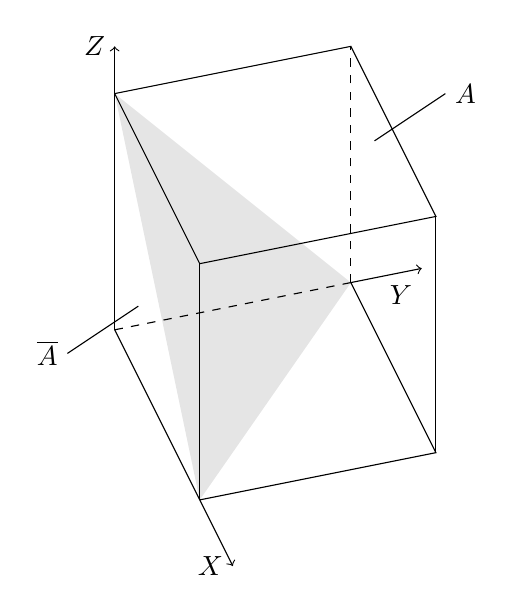
\begin{tikzpicture}[scale=3]
        \def \Ax {0.36};
        \def \Ay {-0.72};
        \def \Bx {1};
        \def \By {0.2};
        \def \Cx {0};
        \def \Cy {1};

        % грань
        \path [fill=gray!20] (\Ax, \Ay) -- ( \Bx, \By ) -- ( \Cx, \Cy );

        % оси
        \draw [->] ( 0, 0 ) -- ( 0.5, -1 ) node [left] at ( 0.5, -1 ) {$X$};
        \draw [dashed] ( 0, 0 ) -- ( \Bx, \By );
        \draw [->] ( \Bx, \By ) -- ( 1.3, 0.26 ) node [below left] at ( 1.3, 0.23 ) {$Y$};
        \draw [->] ( 0, 0 ) -- ( 0, 1.2 ) node [left] at ( 0, 1.2 ) {$Z$};

        % нижние рёбра
        \draw ( \Ax, \Ay ) -- ( \Ax + \Bx, \Ay + \By ) -- ( \Bx, \By );
        % верхние рёбра
        \draw ( \Cx, \Cy ) -- ( \Cx + \Ax, \Cy + \Ay ) -- ( \Cx + \Ax + \Bx, \Cy + \Ay + \By ) -- ( \Cx + \Bx, \Cy + \By ) -- ( \Cx, \Cy );
        % вертикальные рёбра
        \draw [dashed] ( \Bx, \By ) -- ( \Bx + \Cx, \By + \Cy );
        \draw ( \Ax, \Ay ) -- ( \Ax + \Cx, \Ay + \Cy );
        \draw ( \Ax + \Bx, \Ay + \By ) -- ( \Ax + \Bx + \Cx, \Ay + \By + \Cy );

        % cобытия
        \draw ( 1.1, 0.8 ) -- ( 1.4, 1 ) node [right] at ( 1.4, 1 ) {$A$};
        \draw ( 0.1, 0.1 ) -- ( -0.2, -0.1 ) node [left] at ( -0.2, -0.1 ) {$\overline{A}$};
    \end{tikzpicture}
    \caption{Множества $A$ и $\overline{A}$.}
    \label{figure:lesson_3:143:cube}
\end{figure}

Геометрическая мера $\mu \left ( \overline{A} \right )$ представляет собой объём пирамиды $OABC$ (рисунок \ref{figure:lesson_3:143:pyramid}):
\begin{equation}
    \mu \left ( \overline{A} \right )
    = \frac{1}{3} \cdot S_{ABC} \cdot \modulus{OH} ,
\end{equation}
где $S_{ABC}$ --- площадь основания пирамиды (треугольника $\triangle ABC$) и $OH$ --- её высота.

\begin{figure}
    \centering
    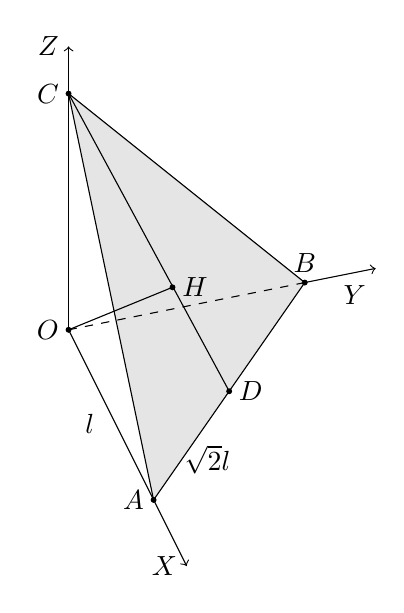
\begin{tikzpicture}[scale=3]
        \def \Ax {0.36};
        \def \Ay {-0.72};
        \def \Bx {1};
        \def \By {0.2};
        \def \Cx {0};
        \def \Cy {1};
        \def \Dx {0.5*\Ax + 0.5*\Bx};
        \def \Dy {0.5*\Ay+ 0.5*\By};
        \def \Hx {0.44};
        \def \Hy {0.18};

        % грань
        \path [fill=gray!20] ( \Ax, \Ay ) -- ( \Bx, \By ) -- ( \Cx, \Cy );

        % оси
        \draw [->] ( 0, 0 ) -- ( 0.5, -1 ) node [left] at ( 0.5, -1 ) {$X$};
        \draw [dashed] ( 0, 0 ) -- ( \Bx, \By );
        \draw [->] ( \Bx, \By ) -- ( 1.3, 0.26 ) node [below left] at ( 1.3, 0.23 ) {$Y$};
        \draw [->] ( 0, 0 ) -- ( 0, 1.2 ) node [left] at ( 0, 1.2 ) {$Z$};

        % основание
        \draw ( \Ax, \Ay ) -- ( \Bx, \By ) -- ( \Cx, \Cy ) -- ( \Ax, \Ay );

        % образующая
        \node [left] at ( 0.15, -0.4 ) {$l$};
        % сторона основания
        \node [right] at ( 0.45, -0.55 ) {$\sqrt{2} l$};

        % точки
        \draw [fill] ( 0, 0 ) circle [ radius = 0.01 ] node [ left ] at ( 0, 0 ) {$O$};
        \draw [fill] ( \Ax, \Ay ) circle [ radius = 0.01 ] node [ left ] at ( \Ax, \Ay ) {$A$};
        \draw [fill] ( \Bx, \By ) circle [ radius = 0.01 ] node [ above ] at ( \Bx, \By ) {$B$};
        \draw [fill] ( \Cx, \Cy ) circle [ radius = 0.01 ] node [ left ] at ( \Cx, \Cy ) {$C$};
        \draw [fill] ( \Dx, \Dy ) circle [ radius = 0.01 ] node [ right ] at ( \Dx, \Dy ) {$D$};
        \draw [fill] ( \Hx, \Hy ) circle [ radius = 0.01 ] node [ right ] at ( \Hx, \Hy ) {$H$};

        % высота в основании
        \draw ( \Cx, \Cy ) -- ( \Dx, \Dy );
        % высота в пирамиде
        \draw ( 0, 0 ) -- ( \Hx, \Hy );
    \end{tikzpicture}
    \caption{Пирамида $\overline{A}$.}
    \label{figure:lesson_3:143:pyramid}
\end{figure}

Основание пирамиды --- равносторонний треугольник $\triangle ABC$, длину стороны можно вычислить из прямоугольного треугольника $\triangle AOB$,
в котором катеты $AO$ и $BO$ имеют длину $l$, а искомая гипотенуза $AB$ имеет длину:
\begin{equation}
    \modulus{AB} = \sqrt{ \modulus{AO}^2 + \modulus{BO}^2 } = \sqrt{2} l.
\end{equation}
Высота $CD$ в равностороннем треугольнике $\triangle ABC$ имеет длину:
\begin{equation}
    \modulus{CD}
    = \frac{\sqrt{3}}{2} \cdot \modulus{AB}
    = \frac{\sqrt{3}}{2} \cdot \sqrt{2} l .
\end{equation}
Таким образом, площадь основания:
\begin{equation}
    S_{ABC}
    = \frac{1}{2} \cdot \modulus{AB} \cdot \modulus{CD}
    = \frac{1}{2} \cdot \sqrt{2} l \cdot \frac{\sqrt{3}}{2} \sqrt{2} l
    = \frac{\sqrt{3}}{2} l^2 .
\end{equation}
Длина высоты $OH$ пирамиды определяется из прямоугольного треугольника $\triangle CHO$, в котором гипотенуза $OC$ имеет длину $l$ и катет $CH$
имеет длину $\frac{2}{3} \cdot \modulus{CD}$:
\begin{equation}
    \modulus{OH}
    = \sqrt{l^2 - \left ( \frac{2}{3} \frac{\sqrt{3}}{2} \sqrt{2} l  \right )^2}
    = \sqrt{l^2 - \frac{4}{9} \frac{3}{4} 2 l^2}
    = l \sqrt{1 - \frac{6}{9}}
    = l \sqrt{1 - \frac{2}{3}}
    = l \sqrt{\frac{1}{3}}
    = \frac{l}{\sqrt{3}} .
\end{equation}

Таким образом, объём пирамиды:
\begin{equation}
    \mu \left( \overline{A} \right)
    = \frac{1}{3} \cdot \frac{\sqrt{3}}{2} l^2 \cdot \frac{l}{\sqrt{3}}
    = \frac{1}{6} l^3 ,
\end{equation}
и объём множества $A$:
\begin{equation}
    \mu \left ( A \right )
    = \mu \left ( \Omega \right ) - \mu \left ( \overline{A} \right )
    = l^3 - \frac{1}{6} l^3
    = \frac{5}{6} l^3 .
\end{equation}

Вероятность события $A$:
\begin{equation}
    \probability{A}
    = \frac{\mu \left ( A \right )}{\mu \left ( \Omega \right )}
    = \frac{\frac{5}{6} l^3}{l^3}
    = \frac{5}{6} .
\end{equation}

\subsection*{Ответ:}
$\frac{5}{6}$.

\section*{Задачи для самостоятельного решения}

Из раздела 18 сборника задач Ефимова и Поспелова.
\begin{enumerate}
    \item На занятии: 144, 151, 158.
    \item Дома: 139, 145, 147, 154, 157.
\end{enumerate}

Из сборника задач типового расчёта Чудесенко: 5, 6, 7.